\documentclass{article}
\usepackage{statsm254,amsmath,abraces}

\usepackage[makeroom]{cancel}


%% the format for the lecture environment is
% \begin{lecture}{lecture number}{lecture title}{scribe(s)}{lecture date}
\begin{lecture}{17}{Lecture 17 - Sampling Methods}{Harry Yang, Christina Burghard}{ 5/31/2017 }


\section{Canonical Correlation Analysis (CCA)}
Dimentionality Reduction for two sets of variables.
e.g. 
n = 40 mice,
r = 120 gene expression levels associated with nutrition,
s = 21 fatty acids' concentration 

 \begin{center}
	X = Gene expression matrix (40 x 120)
	
	Y = Concentration matrix (40 x 21)
\end{center}

CCA seeks linear transformation:

\begin{center}
	$ g_{(120 \times 1)} \in R^r$ 
	
	$ h_{(21 \times 1)} \in R^s $
\end{center}

so that $Cor(X-g, Y-h)$ is maximized.

$(g_1,h_1) = 1^{st}$ canonical correlation vector
$\ldots$ 
$(g_k, h_k) = k^{th}$ canonical correlation vector 
\subsection{Algirothm}
 
$ S_{11} = \hat{Cov(x)} , S_{22} = \hat{Cov(y)} = \frac{1}{n} Y^T Y $ if every column of Y is centered, $ S_{12} = \hat{Cov(x,y)}, S_{21} = \hat{Cov(Y,X)}$
\begin{center}
$ (g_k, h_k) = argmax_{g,h}( g^T S_{12} h / \sqrt{g^T S_{11} g \cdot h^T S_{22} h})$ \\

where $g^T S_{11}g_j = 0, h^T S_{22} h_j = 0, j = 0 \dots k-1$
\end{center}


\section{Simulation Methods}
\subsection{Monte Carlo Method}
Goal: to evaluate a parameter $\theta = E[f(x)] $ for $X \sim P$, where $P$ is 
the target distribution.

For example,
\begin{align}
	P = N(\mu, \sigma^2)
\end{align}
where
$\mu = E[x]$ and $ \sigma^2 = E[(x-\mu)^2]$.


For example, how to calculate the posterior mean if we choose a prior such that 
the posterior doesn't have a nice distribution function?

\begin{enumerate}
	\item Direct (naive) Monte Carlo
	
	Sample $x_i$ as independent and identically distributed from $P$
	
	Take the average $\hat{\theta} = \frac{1}{n} \sum_{i = 1}^{n}f(x_i)$
	
	Find the 95\% conifdence interval, eg $E[x]$
	
	The indicator function is $E[I(x>c)]$ \newline
	
	This is useful for:
	\begin{itemize}
		\item Bayesian inference (from the posterior)
		\item High-dimensional parameter space
		\item When there is no analytic form of the target distribution $P$
	\end{itemize}
	
	Example: $X$ and $Y$ are independent random variables from $Unif(0,1)$. What is 
	$P(X^2 + Y^2 \geq 1)$?
	
	\begin{figure}[h]
		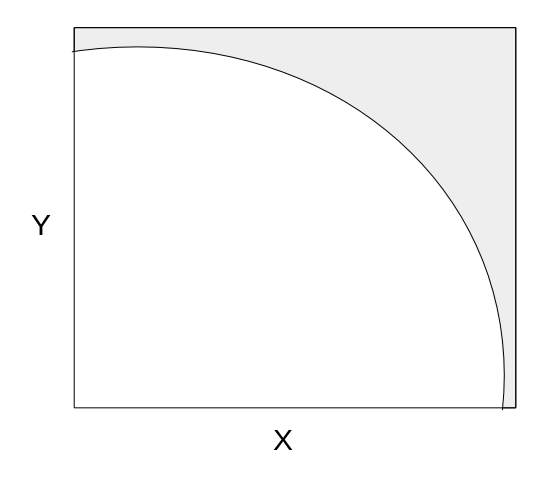
\includegraphics[scale = 0.4]{direct_MC_ex1.png}
		\centering
		\label{fig:2}
		\caption{The white area is $\frac{\pi}{4}$,  the grey region is $1-\frac{\pi}{4}$ , which 
			is equal to the probability.}
	\end{figure}
	
	
	We draw $X_i \sim U(0,1), y$ and $ Y_i \sim i = 1,...,n$
	
	$I(X_i^2+Y_i^2 \geq 1) \longrightarrow 0$ or $1$
	
	As n increases, see if the estimate approaches $1- \frac{\pi}{4}$.
	
	\item How to simulate from a distribution
	
	Theorem: let $ U \sim Unif(0,1)$ , and a distribution has a known cumulative 
	distribution function ( CDF) with inverse.
	
	Let $ X = F^{-1}(U)$, then $ X \sim F$
	
	\begin{align}
		\mathbb{P}(X \leq x) = \mathbb{P}(F^-1(U) \leq x) = \mathbb{P}(U \leq F(x)) 
		\longrightarrow X \sim F = F(x)
	\end{align}
	
	e.g.: (using R function rnorm) 
	if $X \sim F, F(x) = \mathbb{P}(X \leq x)$. We can use $U$ to project $x$.
	
	Example: To sample $X_1, ... , X_n \sim Exponential(1)$:
	\begin{itemize}
		\item In R: rexp(n,1) (use set.seed(0) in order to make this replicable)
		
		\item Manually: sample $ U_1, ... , U_n \sim Unif(0,1)$
		
		CDF of Exp(1):
		
		$F(x) = 1 - e ^{-x}, x \geq 0$ \newline
		$\longrightarrow F^{-1}(x) = -\log(1-x), x \in[0,1]$
		
		Let $X_i = -\log(1-U_i)$
		
		Then $X_1, ... ,X_n ~ Exp(1)$
	\end{itemize}
	
	\item Rejection Method \cite{vonNeuman1951}
	Setting:
	\begin{enumerate}
		\item We want to sample from a target distribution with density $\pi(x)$. 
		\item The density is known to a constant $l(x) = C\pi(x)$ , where $l$ is known, 
		and $C$ and $\pi(x)$ are unknown.
		\item We can construct 
		\begin{enumerate}
			\item an envelope function, $g(x)$
			\item a constant $m$ such that $mg(x) \geq l(x) \forall x...$
			
			\begin{figure}[h]
				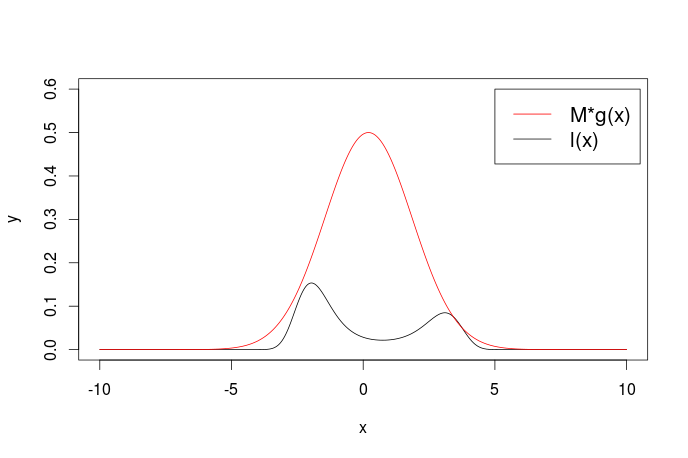
\includegraphics[scale = 0.5]{envelope.png}
				\centering
				\label{fig:3}
				\caption{Here the grey line is $l(x)$ and the black line is $m \ast g(x)$.}
			\end{figure}
			
		\end{enumerate}
		Procedure:
		\begin{enumerate}
			\item Draw a sample point from $g(x)$ and compute the ratio $ r = 
			\frac{l(x)}{mg(x)} \in[0,1]$. (Because $g(x)$ is normal, it's easy to draw a 
			sample.)
			\item Flip a coin with probability of success = $r$, or draw $y \sim 
			Bernoulli(r)$.
			
			If $y = 1$, keep $x$. Otherwise, discard $x$.
			\item Repeat step 1 until the $n^{th}$ sample is accepted.
		\end{enumerate}
		The result of this is that if the sample point from the envelope function is 
		further from the target distribution, it will have a higher ratio and is more 
		likely to be discarded.
	\end{enumerate}
	
\end{enumerate}


\section{Rejection Method}
Goal: To sample from a target distribution with density ${\pi}(x)$ which is unknown. Sampling from a cdf requires the inverse function, which is often difficult to obtain, so for those cases, the rejection method is convenient. The target function can be represented as:
\begin{center}
$l(x) = c \cdot \pi(x)$
\end{center}
where $\pi(x)$ and $c$ are unknown and $l(x)$ is known but difficult to integrate. The approach used by this method is to construct an envelope function $g(x)$ which is known and has a simple, known distribution form (e.g. normal density) such that:
\begin{center}
$m \cdot g(x) \geqslant l(x) \hspace{1cm} \forall x$
\end{center}
\begin{figure}[h]
  \centering\textbf{}
  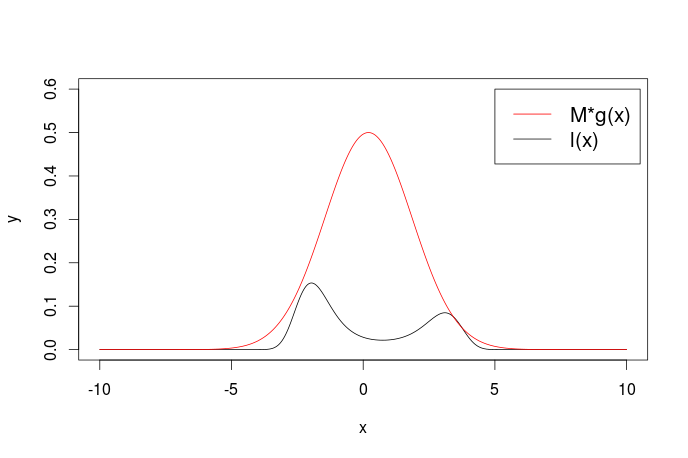
\includegraphics[width=9cm]{envelope.png}
  \caption{Target and Envelope function}
\end{figure}

\subsection{Algorithm}
To obtain a sample of n data points. 
\begin{itemize}
\item Draw a point $x_i$ from the envelope function $g(x)$ so that $x_i \sim g(x)$. 
\item Compute the ratio r:
\begin{center}
$r = \dfrac{l(x_i)}{m \cdot g(x_i)}$
\end{center}
\item Draw $z$ as a Bernoulli trial with probability $r$, i.e. $z \sim bernoulli(r)$ (rbinom function in R). If $z = 1$ keep $x_i$, else discard $x_i$. 
\item Repeat until you get n data points. 
\end{itemize}

\subsection{Why does it work?}

\begin{equation*}
\left.
\begin{aligned}
	\text{Let } z = 
\end{aligned}
\right.
	\begin{cases}
	1 & \text{if } X \sim g(x) \text{ is accepted}\\
	0 & \text{ otherwise}
	\end{cases}	
\end{equation*}
Then \\ 
\begin{eqnarray*}
	p(z=1) & =\int p(z=1 , X = x) dx \\[0.8em]
	& =\int p(z=1 \mid X = x) \cdot g(x) dx \\[0.8em]
	& = \int \dfrac{l(x)}{m \cdot \cancel{g(x)}} \cdot \cancel{g(x)} dx \\[0.8em]
	& = \int \dfrac{c \cdot \pi(x)}{m} dx = \dfrac{c}{m} \\[0.8em]
\end{eqnarray*}
% \begin{align*}
% 	p(z=1) & =\int p(z=1 , X = x) dx \\[0.8em]
% 	& =\int \underbrace{p(z=1 \mid X = x)}_{\mathclap{\text{bernoulli (r)}}} \cdot g(x) dx \\[0.8em]
% 	& = \int \dfrac{l(x)}{m \cdot \cancel{g(x)}} \cdot \cancel{g(x)} dx \\[0.8em]
% 	& = \int \dfrac{c \cdot \pi(x)}{m} dx = \dfrac{c}{m} \\[0.8em]
% \end{align*}

Therefore, the probability of a value being kept for the sample is equal to the target distribution $\pi(x)$  \\ 
\begin{align*}
	p(X = x \mid z=1) & =\dfrac{p(X=x , z=1)}{p(z=1)} \\[0.8em]
	& = \dfrac{p(X=x \mid z=1) \cdot g(x)}{p(z=1)}\\[0.8em]
	& = \dfrac{\dfrac{l(x)}{m \cdot g(x)} \cdot g(x)}{\dfrac{c}{m}} = \pi(x) \\[0.8em]
\end{align*}

\subsection{How to choose a good envelope}
Consider the distribution $\pi(x)$ 
\begin{align*}
	\pi(x) \propto \Phi(x) \cdot I(x > c) \\[0.8em]
	\text{where } \Phi \sim \mathcal{N}(0,1)
\end{align*}

\begin{itemize}
\item \textbf{Method 1} \\
For the first method we choose the Normal Gaussian distribution as the envelope function $g(x) = \Phi(x)$ (Figure 2).\\
\begin{figure}[h]
  \centering
  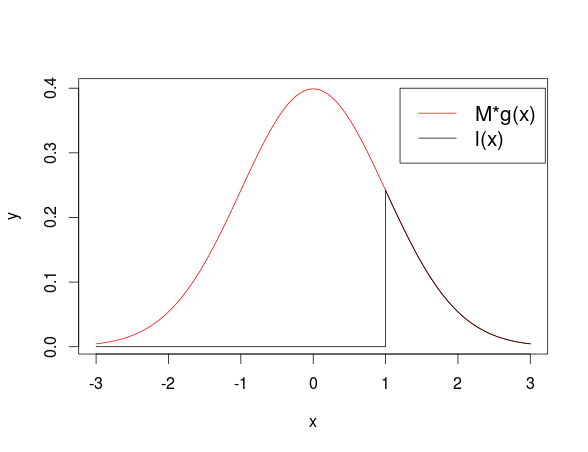
\includegraphics[width=9cm]{method1.png}
  \caption{Target and Envelope function(Normal Distribution), $c = 1$.}
\end{figure}
\begin{equation*}
\left.
\begin{aligned}
	r = 
\end{aligned}
\right.
	\begin{cases}
	0 & \text{if  } x \leq c \\
	1 & \text{if  } x > c\\
	\end{cases}	
\end{equation*}

For this approach, for high values of $c$, the acceptance rate is very low. This implies that a lot of points need to be rejected before completing the sample with n points. This approach is not very effective. 
\item \textbf{Method 2} \\
For the second approach, we consider the exponential density $g(x) = \lambda e^{- \lambda (x-c)}$ where $x \in [c, \infty]$ . 
\begin{figure}[h]
  \centering
  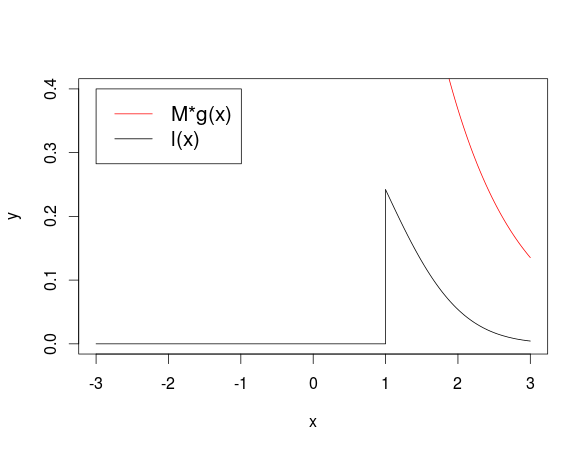
\includegraphics[width=9cm]{method2.png}
  \caption{Target and Envelope function(Exponential), lambda = 1.}
\end{figure}
This approach is more effective since we can draw samples from the defined range of $x$. and for larger $c$ values, it has a higher acceptance rate (Figure 3). \\
\\
Ok, but what is $\lambda$ ? \\
Find the smallest $M$ such that:
\begin{align*}
	M &\geqslant \dfrac{\Phi(x)}{g(x)} \hspace{1cm} \forall x \geqslant c \\[0.8em]
	M &\geqslant \dfrac{\dfrac{1}{\sqrt{2\pi}}e^{-\dfrac{x^2}{2}}}{\lambda e^{- \lambda (x-c)}} = \dfrac{1}{\lambda\sqrt{2\pi}}e^{- \left( \dfrac{x^2}{2} - \lambda x - \lambda c \right)}\\[0.8em]
\end{align*}
For the expression above, we need to find the values of $x$ that maximizes the whole expression to guarantee the inequality holds. To find this value, we need to find the $x$ that minimizes $  \dfrac{x^2}{2} - \lambda x - \lambda c $ and is equal or greater than $c$ which is $x = \lambda$ \\ 
\begin{align*}
	M &= \max_{x>c} \dfrac{1}{\lambda\sqrt{2\pi}}e^{- \left( \dfrac{x^2}{2} - \lambda x - \lambda c \right)}=\dfrac{1}{\lambda\sqrt{2\pi}}e^{ \left( \dfrac{\lambda^2}{2} - \lambda c \right)}\\[0.8em]
\end{align*}
Now we have M as a function of $\lambda$. To find the smallest $M$ we need to find the value of $\lambda$ that minimizes that function.  
\begin{align*}
	\lambda &= \argmin_{\lambda} M(\lambda) = \argmin_{\lambda} \dfrac{1}{\lambda\sqrt{2\pi}}e^{ \left( \dfrac{\lambda^2}{2} - \lambda c \right)} \\[0.8em]
	\lambda &= c
\end{align*}
\end{itemize}
Acceptance rate:
\begin{center}
 \begin{tabular}{|c c c c|} 
 \hline
 Method & $c=-1$ & $c=2$ & $c=3$ \\ [0.5ex] 
 \hline\hline
 1 & 0.84 & 0.02 & 0.0009 \\ 
 \hline
 2 & 0.57 & 0.88 & 0.96 \\ 
 \hline
\end{tabular}
\end{center}
From the table above we can see that the exponential envelope function has a higher acceptance rate for larger values of $c$, therefore it's a more efficient approach. \\
A good envelope function have the following properties:\\
\begin{itemize}
\item It should be easy to sample from
\item It should be easy to construct (find M)
\end{itemize}
\begin{thebibliography}{10}
	\bibitem{vonNeuman1951}
	J. von Neumann, ``Various techniques used in connection with random digits. 
	Monte Carlo methods", \emph{Nat. Bureau Standards}, 12 , pp. 36–38, 1951.
\end{thebibliography}
\end{lecture}
\theend	